\chapter{Monte-Carlo Simulations}
\label{chap::MC}

\chapterquote{You're always one spin away form winning. Don't stop...}%
{Iain Mclean, when asked about healthy habits.}
Monte-Carlo (MC) simulations are a key part of any ATLAS physics analysis as they provide a reference to data with defined physics inputs in order to understand the detector response. Generation of the MC events start: the Matrix Element (ME) for the hard-scattering process of interest. However, with any hard-scattering event comes soft emissions that if would be too computationally intensive to calculate in the same way as the hard scattering events and so these emissions are simulated using a Parton Shower (PS). The resulting partons then under go hadronization, using a non-perturbative model. Remnants of the protons after collisions can also enter the detector volume and interact further, or decay forming part of the underlying event. As each bunch crossing results in around 30-40 other interactions, pile-up also needs to be modelled. Lastly the detectors effects must be taken into account and the final-state particles must be passed through a simulation of the ATLAS detector geometry. An illustration of these stages can be seen in Figure \ref{fig:tth_MC}.

\begin{figure}
    \centering
    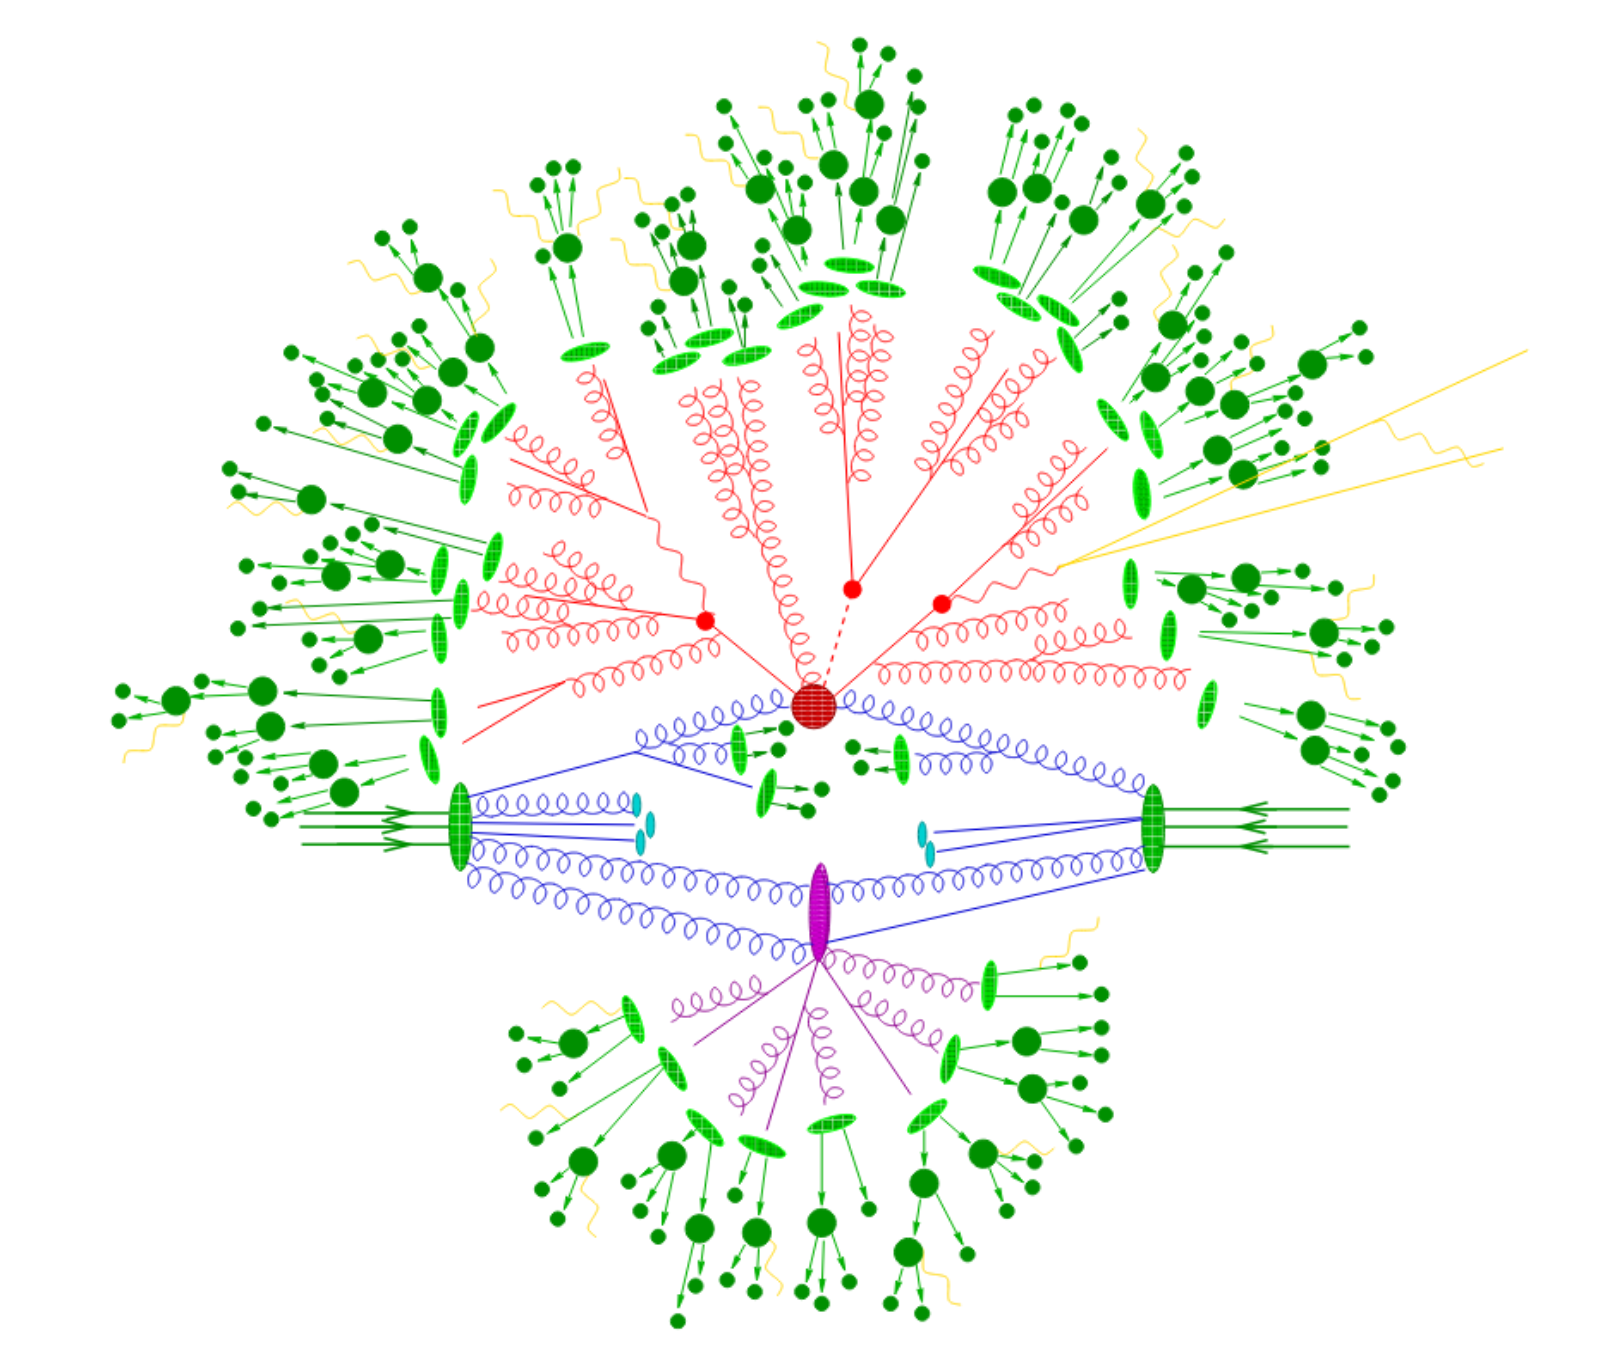
\includegraphics[width=0.7\linewidth]{Section_Monte_carlo/tth_mc_event.png}
    \caption{Depiction of a $t\bar{t}H$ event decaying semi-leptonically produced with an event
generator \cite{ttH_MC_pic}.}
    \label{fig:tth_MC}
\end{figure}

\section{Matrix Element Generation}
The cross section of all QCD interactions requires knowledge of the strong coupling constant, $\alpha_s$ which is inversely proportional logarithm of the to the energy of a given interaction. Considering a $pp$ collision, these collisions involve a mix of interactions at different energy scales. At low energies ($\alpha_s>1$)  higher-order perturbative contributions to the collision cross-section do not converge and thus the calculation cannot be solved using Equation \ref{cross_sec_expan}.
\begin{equation}\label{cross_sec_expan}
    \hat{\sigma}_{ab\rightarrow X}= \hat{\sigma}_0 + \alpha_S \hat{\sigma}_1 +\alpha_S^2 \hat{\sigma}_2\ +\  ...,
\end{equation}
where $\hat{\sigma}_0$ describes the Leading Order (LO) (or tree level) contribution, $\alpha_S \hat{\sigma}_1$ are the Next-to-Leading Order (NLO) corrections and so on. At the next stage, in the PS, the real emissions from the higher order $\alpha_S$ term are described either as Initial State Radiation (ISR) and Final State Radiation (FSR) we discuss this more in Section \ref{PS}.
\subsection{Factorisation Theorem}
In order to combat the non-perturbative nature of high order $\alpha_S$ terms, the factorisation theorem is deployed \cite{factorisation_therome}. This states that by defining a factorisation energy scale ($\mu_f$) as a crossing point between perturbative and non-perturbative behaviour the cross-section calculation can be factorised into high-energy and low-energy and so can be solved independently. A production cross-section of some process X from a proton-proton collision can be given by:
\begin{equation}
    \sigma_{pp\rightarrow X} = \sum_{i,j \in  \{q,\bar{q},g\}} \int dx_1 \int dx_2 f_i(x_1,\mu_f^2)f_j(x_2,\mu_f^2)\hat{\sigma}_{ij},
\end{equation}
where $i$ and $j$ denote the parton species of the incident particle, $f_i(x_{1(2)},\mu_f^2)$ is the Parton Distribution Function (PDFs), and $\hat{\sigma}_{ij}$ is the partonic cross-section for parton $i,j$ to produce $X$.
\subsection{Parton Distribution Functions}
In a proton we have three valance quarks ($uud$) and a sea of other miscellaneous quarks and gluons which aren't fully bound at high energies. Each one of these partons carry some fraction of the protons total momentum in order to described the \"who has what" problem this description of a proton faces we introduce the PDF. The PDF, $P_i(x)$, gives the probability for finding a parton of type $i$ carrying a fraction $x$ of the proton's momentum. These distributions are relevant at interaction scales typically ranging from 100 to 1000 GeV, where high-energy collisions probe the internal structure of the proton. Since PDFs arise from non-perturbative QCD dynamics, they cannot be calculated directly from first principles and are instead parametrised using experimental data. However, their dependence on the energy scale is predictable and is governed by the DGLAP evolution equations, which describe how PDFs change as the probing scale increases \cite{DGLAP1,DGLAP2,DGLAP3}.
\\
\\
An important part of the factorisation scheme is how b-quarks are treated in QCD processes. There are two main approaches. In the Four Flavour Scheme (4FS), b-quarks are considered massive and too heavy to appear in the initial state. As a result, they don't have a parton distribution function (PDF) and are excluded from the running of $\alpha_S$. This approach is better for low-energy processes where the b-quark mass matters. In contrast, the Five Flavour Scheme (5FS) is used at higher energies, where the b-quark mass becomes negligible. Here, b-quarks are treated as massless, included in the proton’s structure via a PDF, and contribute to $\alpha_S$running like the lighter quarks.

\section{Parton Shower} \label{PS}
Once we have generated our hard scattering process, we then need to apply parton shower effects, where the high-energy quarks and gluons produced begin to radiate further particles. Each parton has a finite probability of splitting, such as a gluon decaying into a quark-antiquark pair ($g \to q\bar{q}$), a quark emitting a gluon ($q \to gq$), or a gluon splitting into two gluons ($g \to gg$). Parton shower generators calculate these probabilities at different scales, simulating the step-by-step radiation as partons lose energy. This process continues until the evolution reaches scales of order $1~\text{GeV}$, where perturbative QCD is no longer valid and the simulation hands over to hadronisation models to form stable particles. Radiation is typically modelled as two separate but conceptually similar cascades FSR and ISR.\\
\\
FSR occurs after the hard scattering, where outgoing high-virtuality partons branch as they propagate towards lower energies. The probability that a parton does not emit further radiation between two evolution scales $Q$ and $Q_0$ is given by the Sudakov form factor,
    \begin{equation}
        \Delta(Q^2, Q_0^2) = \exp \left[ - \int_{Q_0^2}^{Q^2} \frac{\mathrm{d}k^2}{k^2} \int \mathrm{d}z \, P(z) \right],
    \end{equation}
where $P(z)$ is the relevant Altarelli-Parisi splitting function \cite{Lonnblad2005PartonShowers}. Where the emission probability grows as the scale decreases, and the Sudakov factor acts as a survival probability against emission.\\
\\
ISR describes radiation from the incoming partons before the hard scattering. ISR is typically implemented via backward evolution, starting from the hard-scattering scale and evolving to lower scales, reconstructing possible emissions in reverse. The emission probability is again governed by a Sudakov factor, but here the splitting probabilities are weighted by the ratio of parton distribution functions (PDFs). This accounts for the fact that, when evolving backward, certain branchings are suppressed if the required parent parton is rare in the proton at the relevant momentum fraction.\\
\\
In both cases, the Sudakov form factor ensures the probabilistic consistency of the shower: it enforces that exactly one branching occurs at each step, with the intervals between emissions determined by the no-emission probability. The shower evolution thus resums large logarithms associated with soft and collinear radiation, providing a bridge between the hard process and the hadronisation stage.


\section{Hadronisation}
Once we have reached the showering threshold, the parton energy is low enough that quarks begin to form bound states, resulting in the formation of hadrons, a process known as hadronisation. There are two main models used to simulate hadronisation: the cluster fragmentation model and the Lund string model \cite{Lund_string}. The cluster fragmentation model, used by SHERPA, works by first forcing gluons to split into quark–antiquark pairs \cite{Cluster|_frag}. These quarks then group into colour-neutral clusters, which subsequently decay into hadrons. In contrast, the Lund string model, used by PYTHIA, treats the colour field between partons as a string that stretches as they move apart. When the string’s potential energy becomes large enough, it breaks, creating new quark–antiquark pairs. This process repeats until all partons are converted into colourless hadrons. Both models are based on the principle of Local Parton–Hadron Duality, which assumes that the momentum and quantum number flow at the hadron level follows that of the parton level \cite{PHD}.

\section{Underlying Event and Multi-Parton Interactions}
The Underlying Event (UE) refers to all the activity in a proton–proton collision that is not part of the main hard scattering, including remnants of the incoming protons, soft radiation, and additional parton–parton scatterings known as Multi-Parton Interactions (MPI). These MPIs occur when multiple partons from each proton interact simultaneously, often producing low-momentum particles. Like the products of the hard scatter, the partons from the UE and MPI also carry colour charge and therefore must form colour-bound states. They undergo hadronisation through the same mechanisms, such as the Lund string or cluster model—forming hadrons that contribute to the soft particle activity observed in the final state of a collision event.

\section{Pile up}
Pile-up is modelled by overlaying additional soft minimum-bias events (representing random pp collisions) on top of the hard-scatter event, These are generated using \verb|PYTHIA8| \cite{PYTHIA8}. The number of contributions can sometimes not match data and so need to be re-weighted to do so, this is called pile-up re-weighting.

\section{Detector simulation}
The final step in the Monte Carlo event generation process is to pass the simulated events through a detector simulation, which models how the final-state particles interact with the detector hardware. For the ATLAS experiment, this is done using \verb|GEANT4|, a detailed toolkit that simulates the passage of particles through the detector systems \cite{GEANT4_1,GEANT4_2}. The tools includes simulating: interactions with materials, energy loss, scattering, and detector responses. Accurately modelling these effects requires significant computational effort. As a result, the full \verb|GEANT4|-based simulation is often the most time-consuming part of the entire MC workflow, representing the dominant share of CPU resources used in sample production for ATLAS analyses.\\
\\
An intermediate option is \verb|ATLFAST-II|, which combines full \verb|Geant4| simulation for the inner detector and muon spectrometer with the parameterised calorimeter simulation \verb|FastCaloSim|, typically interfaced via \verb|FATRAS|. This hybrid approach delivers an order of magnitude reduction in CPU time compared to the full simulation, while maintaining significantly higher accuracy than the fully parameterised \verb|ATLFAST| model \cite{ATLAS2008_LatfastII,ATLAS2010_FastCaloSim,ATLAS2008_FATRAS}.\\
\\
More recently, \verb|ATLFAST3| has been developed as the next-generation fast simulation platform. By combining traditional FastCaloSim techniques with machine‑learning based calorimeter shower models, it achieves accuracy closer to full \verb|Geant4| simulation while preserving the high-speed performance needed for large event samples \cite{ATLAS2022_AtlFast3}.